\chapter{REVIEW OF RELATED LITERATURE}
{\baselineskip=2\baselineskip
 This chapter focuses on related studies or projects that have provided additional relevant information to the proponent. Section 2.1 presents the theoretical background related to machine learning and mechatronics. Section 2.2 specifies the concept of how the system will classify the eggplants by class based on surface defects, color homogeneity, and shape. Section 2.3 presents a review of literature related to the design of employing machine learning and mechatronic integration in agricultural automation for image-based inspection and mechanical sorting applications. Collectively, these reviewed literatures support the concept presented in this study. 

%-----------------------------------------------------------------------------------------------------------------------
\section{Theoretical Background}
The development of an automated eggplant grading system is fundamentally grounded in the integration of theoretical paradigms of computational intelligence and mechanical control. This framework draws from the convergent disciplines of machine learning and mechatronics to create a cyber-physical system capable of perceiving, deciding, and acting. The following subsections detail the core theories that underpin the image analysis, classification, and physical sorting mechanisms of the proposed system.

\begin{figure}[h]
	\centering
	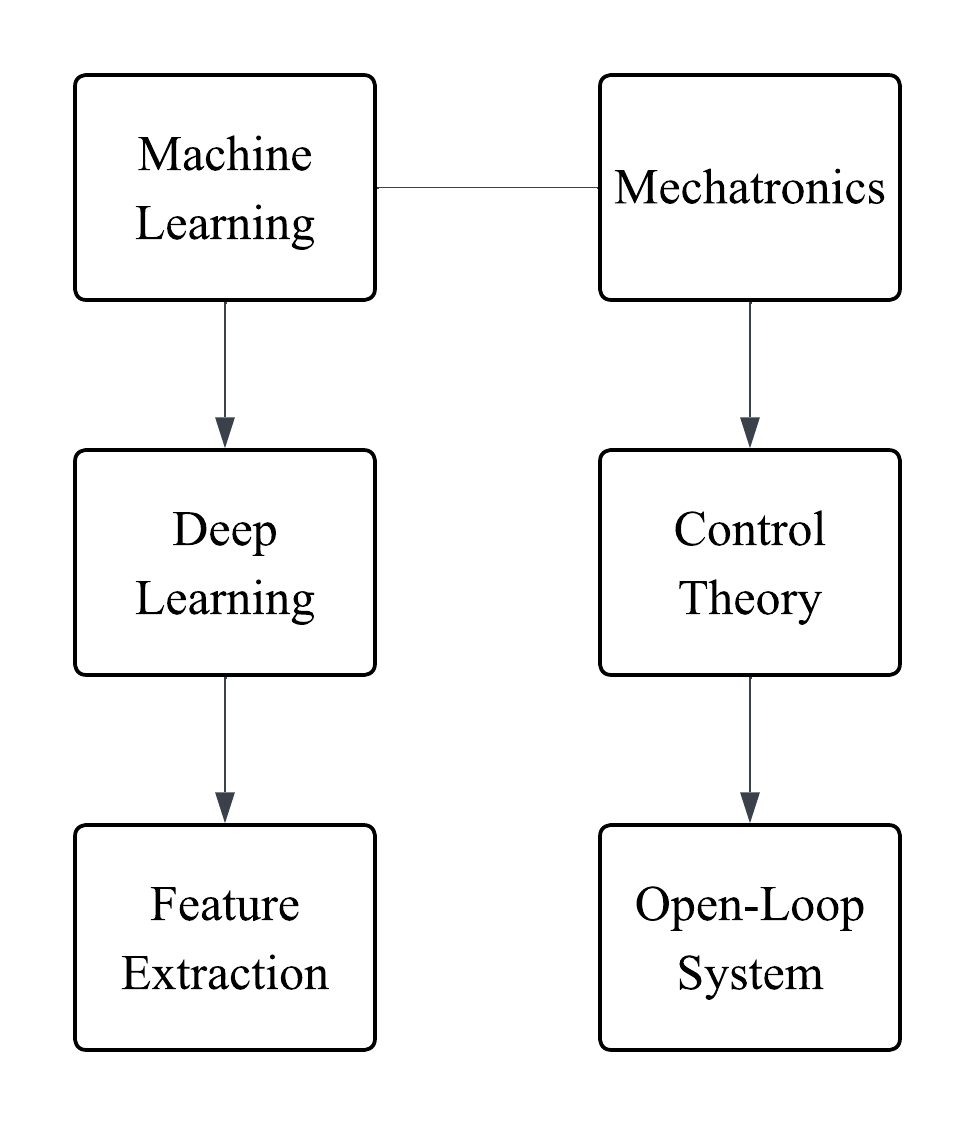
\includegraphics[height=0.4\textheight]{figures/theoreticaldiagram}
	\caption{Theoretical Framework}
	\label{fig:theoreticalframework}
\end{figure}

The development of an automated eggplant grading system is fundamentally grounded in the integrated theoretical paradigms of computer vision, deep learning, and mechatronics. The entire process can be conceptualized through a sequential computer vision pipeline, which moves from image acquisition to physical actuation \citep{szeliski2022computer}. This pipeline begins with the digital image formation theory, where a camera sensor captures light reflectance from objects on a conveyor belt, a common setup in food process engineering \citep{dougherty2020digital}. The stability and quality of this initial stage are paramount, as controlled, diffuse illumination is critical to minimize specular reflections and shadows that can obscure critical features like color and surface defects, thereby ensuring consistent input for subsequent algorithmic processing.

Following acquisition, image pre-processing theories are applied to enhance data quality and standardize inputs. This involves digital signal processing techniques such as noise reduction using Gaussian or median filters \citep{kumar2020comparative} and, crucially, color space transformation. Converting images from the default Red-Green-Blue (RGB) space to Hue-Saturation-Value (HSV) or \textit{CIEL*a*b*} is a well-established step in agricultural product inspection \citep{khan2024intelligent}. The theoretical underpinning for this conversion lies in the decoupling of color information (chrominance) from intensity (luminance) in these spaces, making the extracted color features more robust to minor variations in lighting conditions, which is essential for accurate color-based grading.

The core of the system resides in the theoretical distinction between traditional machine learning and deep learning for feature extraction. Traditional approaches are based on manual feature engineering, drawing from image processing and pattern recognition theory to hand-craft descriptors for color (e.g., histograms, mean values), shape (e.g., aspect ratio, roundness, area), and texture (e.g., using Gray-Level Co-occurrence Matrix (GLCM) or Local Binary Patterns (LBP)) \citep{haralick2007textural,ojala2002multiresolution}. In contrast, deep learning, specifically Convolutional Neural Network (CNN) theory, posits that models can automatically learn a hierarchical representation of features directly from raw pixel data \citep{lecun2015deep,goodfellow2016deep}. The lower layers of a CNN learn generic features like edges and corners, while deeper layers synthesize these into complex, task-specific features relevant to defect identification, thereby eliminating the need for manual feature design.

For the classification task itself, the theoretical models diverge. Machine learning classifiers operate on the principles of statistical learning theory, finding optimal hyperplanes to separate classes or constructing ensembles of decision trees, respectively, based on the handcrafted features \citep{hearst1998support,breiman2001random}. Conversely, an end-to-end deep learning model uses a fully connected output layer with a normalized exponential function (also known as \textit{Softmax}) to perform classification based on the high-level features it learned itself. The theoretical advantage of CNNs is their superior ability to model complex, non-linear relationships in visual data, a capability that has been demonstrated to outperform traditional methods in numerous agricultural applications \citep{bharman2022deep}.

The integrity of any supervised learning system is dependent upon the quality of its labeled dataset. The establishment of a reliable ground truth is a theoretical problem rooted in psychometrics and expert systems. The grading labels for the eggplant images must be derived from standardized agricultural protocols, such as those provided by the United States Department of Agriculture (USDA) or equivalent bodies, which define quality classes based on size, color uniformity, and defect tolerances \citep{USDA2013EggplantStandards}. Locally, the project will utilize the criteria defined by the Philippine National Standard (PNS), and Bureau of Agricultural and Fisheries Product Standards (BAFPS) (specifically the PNS/BAFPS 52:2007), which classifies eggplants into Extra Class, Class I, and Class II based on visual quality, size, and defect tolerances \citep{PNSBAFPS522007_Eggplant,BAFS2019PhilGAP}. To ensure scientific rigor, the concept of inter-rater reliability, often measured by Cohen’s Kappa statistic ($\kappa$), must be applied to quantify the agreement between human experts who label the dataset, thereby validating the consistency of the training labels \citep{mchugh2012interrater,he2022cohens}.

The closed-loop system theory integrates the digital classification with physical actuation. The decision output from the classification model (e.g., a specific grade) is transmitted via a software-to-hardware interface to a Programmable Logic Controller (PLC) or microcontroller \citep{bolton2015programmable}. This triggers a mechatronic actuator, such as a pneumatic pusher or a servo-controlled diverter, which physically sorts the eggplant into its designated bin on the conveyor line. This final stage embodies the principle of cyber-physical systems, where computational intelligence directly controls a physical process to achieve full automation, replicating and potentially surpassing human grading efficiency \citep{lee2008cyber,zhang2022advancements}.

\section{Related Studies}
This section explores existing research and advancements in key areas relevant to the development of the eggplant quality classification and sorting systems. It covers topics such as automated quality grading and sorting systems, image processing techniques, feature extraction, and classification techniques, highlighting their applications and contributions to efficient data processing and real-time quality classification.

\subsection{Automated Quality Grading and Sorting Systems}

The automation of quality grading and sorting represents a critical advancement in postharvest technology, addressing labor shortages, improving consistency, and enhancing operational efficiency. The field has seen significant progress through the development of various machine vision-based systems for a wide range of fruits. These systems typically integrate specialized hardware for fruit handling and imaging with sophisticated software algorithms for quality assessment. The following reviews demonstrate a spectrum of technological approaches, from traditional image processing techniques to advanced deep learning models like CNNs, YOLOv8, and ShuffleNet v2. A common focus is the evaluation of key quality attributes such as surface defects, color, size, mass, and shape, enabling high-speed, automated sorting into commercial grades. 

\sectionsubsub{Design and Experimentation of a Machine Vision-Based Cucumber Quality Grader}

The study designed a novel height difference-free grading mechanism—the fixed tray type—to protect the vulnerable, dense-spined North China type cucumber from damage during automated sorting. The study also introduced a new convolutional neural network architecture named MassNet, which can predict the mass of a cucumber with high accuracy using only a single RGB top-view image, eliminating the need for complex feature extraction. In the mechatronic system, cucumbers were transported on custom-designed trays along a conveyor, with a vision system inside a detection box capturing images triggered by a photoelectric sensor. An electrical control strategy using a PLC ensured real-time synchronization between the predicted grade information and the tray’s position, activating electromagnet-controlled turnouts to direct trays to one of three grading chutes based on mass. For the algorithm, MassNet was developed, incorporating Cross-Stage Partial Connections (CSPC) to enhance feature learning. It was trained on a dataset of 409 cucumber images using the Adam optimizer and MSE loss. The key findings showed that the grader achieved a maximum capacity of 2.3 tonnes per hour. In comparative experiments, MassNet significantly outperformed established models like AlexNet, MobileNet, and ResNet in mass prediction, achieving a MAPE of 3.9\% and a RMSE of 6.7g. In the online grading experiment with 100 cucumbers, the system achieved a high grading efficiency of 93\% at a speed of 60 pieces per minute, with no damage incurred on the cucumbers \citep{liu2024design}.

\begin{figure}[ht]
	\centering
	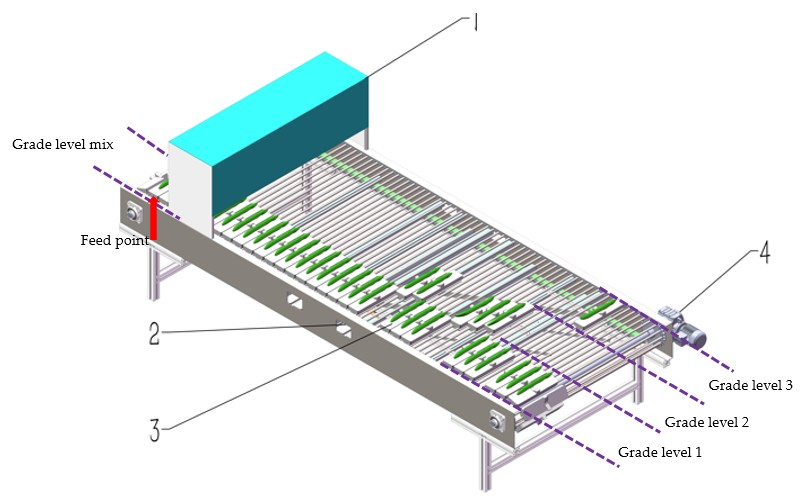
\includegraphics[width=0.7\linewidth]{figures/Liu2024}
	\caption{Structure and grading schematic of the cucumber grading machine \citep{liu2024design}}
	\label{fig:liu2024}
\end{figure}

\sectionsubsub{Design, Prototyping, and Evaluation of a Machine Vision-based Automated Sweetpotato Grading and Sorting System}

The study developed a novel integrated YOLOv8 machine vision-based system for online automated grading and sorting of sweet potatoes. The developed system consisted of two major units: a roller conveyor-based machine vision unit and sorting mechanisms configured on a belt conveyor. The 490$\times$230 mm roller conveyor utilized a chain-rack-gear mechanism to simultaneously transport and rotate sweetpotatoes, and was powered by a parallel shaft gear motor with a speed controller. An enclosed image chamber was assembled on top of the conveyor, housing a downward-facing RGB-D camera and LED lighting to capture multiple views of the rotating samples. A key innovation was the development of a computer algorithm pipeline using YOLOv8 combined with BoT-SORT for real-time instance segmentation and tracking of individual sweetpotatoes, enabling full-surface inspection. This pipeline performed quality grading by estimating size (length and width via ellipse-fitting) and classifying surface defects, then integrating this multi-view data to assign a final grade (Premium, Good, or Fair) based on USDA standards. The sorting mechanism employed two pneumatically-activated linear air cylinders, timed by an IR sensor, to push graded sweetpotatoes into respective bins. The study experimented on 267 sweet potato storage roots of two varieties, Bayou Belle and Orleans. Results demonstrated that system performance was evaluated at three conveyor speeds (4, 8, and 12 cm/s), with a clear trend of decreasing accuracy as speed increased. The sorting mechanisms alone achieved accuracies of 98.9\%, 98.3\%, and 96.9\% at the respective speeds. Correspondingly, the machine vision unit achieved overall grading accuracies of 97.9\%, 95.8\%, and 93.8\% when considering both size and surface defects. The fully integrated system successfully merged these components, achieving overall online sorting accuracies of 97.9\%, 94.8\%, and 92.7\% at the low, medium, and high speeds, thereby validating the prototype’s efficacy for automated sweetpotato grading and sorting \citep{xu2024design}.

\begin{figure}[ht]
	\centering
	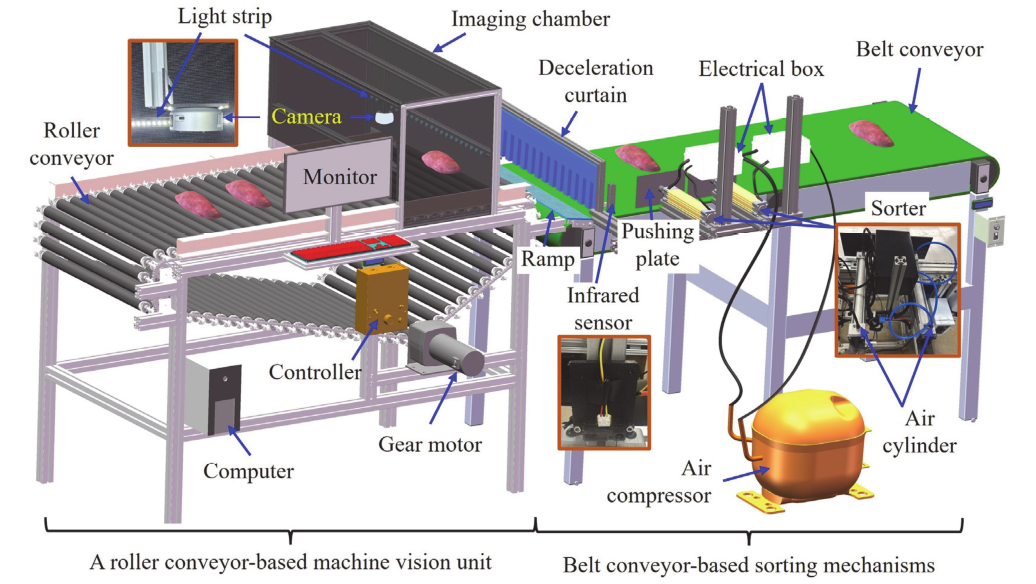
\includegraphics[width=0.7\linewidth]{figures/Xu2024}
	\caption{Scheme of the main hardware elements of the integrated sweetpotato grading and sorting system \citep{xu2024design}}
	\label{fig:Xu2024}
\end{figure}

\sectionsubsub{Research on Citrus Grading System Based on Machine Vision}

The study implemented a citrus grading system based on machine vision, strictly adhering to the Chinese national standard GB/T 12947-2008. The system classified citrus into four grades (Superior, First-class, Second-class, and Other) based on three criteria: transverse diameter (size), colouring rate (proportion of orange-red area), and circularity (shape). The hardware platform utilized a CCD industrial camera, LED lights, and a conveyor belt. For software, images were preprocessed using bilateral filtering and grayscale transformation. The Canny edge detection algorithm was then applied to extract fruit contours. The minimum circumcircle method was used to calculate the diameter (with a conversion ratio of 0.588 mm/pixel) and circularity, while the H component in the HSV colour model and a flood-fill algorithm were used to determine the colouring rate. The key findings from testing five citrus samples showed that the system's diameter measurement had a maximum error of 1.000 mm, a minimum error of 0.006 mm, and all absolute errors were within $\pm$1.5 mm. The system’s grading results for all five samples were 100\% consistent with manual grading based on the national standard. Furthermore, the system demonstrated high computational efficiency, with an average startup time of 0.0798 seconds and stable memory usage averaging 11.203 MB. The study concluded that the system provides an accurate, efficient, and standardized solution for automated citrus grading \citep{xu2025research}.

\sectionsubsub{Development and Evaluation of an Apple Infield Grading and Sorting System}

The study developed and evaluated a compact, high-throughput apple infield grading and sorting system to enable cost-saving pre-sorting of harvested fruit directly in the orchard. The system integrated three key components – pitch-variable screw conveyors that simultaneously singulated, rotated, and transported apples, a machine vision unit that used a single CCD camera to grade apples based on size and color into fresh or processing categories, and a novel paddle sorter activated by a rotary solenoid to divert fruit into the appropriate bins. The vision system involved segmenting the fruit from the background using a two-class linear-discriminant classifier trained on RGB pixel intensities. For size estimation, the system determined the stem-calyx orientation and calculated the maximum equatorial diameter, achieving an error within ±1.8 mm. For color grading, the RGB images were converted to the HSV color space, and the hue channel was analyzed using predefined thresholds to classify each pixel as red, stripe, or green; the final color grade was then determined by the area percentages of these colors, with specific criteria set for different apple varieties. Laboratory testing with Red Delicious and Golden Delicious apples at three system throughputs (7.5, 9.0, and 10.5 apples per second) was conducted. The results demonstrated that the system achieved high intra-lane grading repeatability (above 90\%) and robust inter-lane repeatability (above 81\%). Critically, it caused 45\% bruising damage during the grading and sorting process, with 100\% of tested apples meeting the “Extra Fancy” grade requirement. Furthermore, the system achieved a remarkably high sorting accuracy of over 99\% across all tested throughputs and fruit varieties, demonstrating its robustness and potential for commercial infield application \citep{zhang2021development}.

\sectionsubsub{Multi-Camera-Based Sorting System for Surface Defects of Apples}

The study developed a multi-camera apple sorting system with a rotational mechanism designed to overcome the limitations of single-camera setups by ensuring uniform and accurate imaging of the entire apple surface through a dedicated 180-degree rotation mechanism and three synchronized industrial cameras. The image processing pipeline began with a custom segmentation algorithm that employed pyramid-based downsampling for efficient apple position estimation, followed by a histogram-based analysis in the RGB color space to isolate the fruit from the background using the criteria that red pixel intensity was significantly higher than green and blue, and concluded with cropping to create standardized, background-free input images. To enable real-time processing on embedded hardware (NVIDIA Jetson Nano), the authors utilized a Knowledge Distillation framework, transferring knowledge from a high-performance teacher model (RegNetY-8.0GF) to a compact student model (a lightweight ResNet18), which served as the final CNN classifier. The key findings demonstrated that this approach yielded a highly efficient system, with the distilled student model achieving an inference speed of 0.069 seconds per image and a final sorting accuracy of 93.83\% across 300 apple samples, successfully processing one apple every 2.84 seconds while comprehensively scanning its entire surface \citep{lee2023multi}.

\begin{figure}[ht]
	\centering
	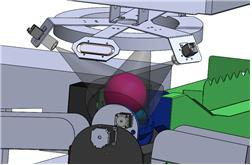
\includegraphics[width=0.45\linewidth]{figures/Lee2023_1} 
	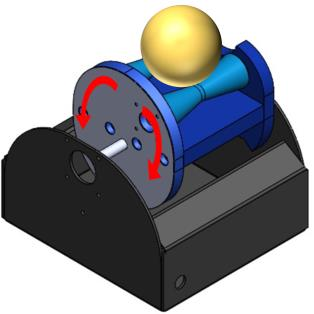
\includegraphics[width=0.3\linewidth]{figures/Lee2023_2}
	\caption{Camera structure and rotation mechanism \citep{lee2023multi}}
	\label{fig:Lee2023}
\end{figure}

\sectionsubsub{Infield Apple Detection and Grading Based on Multi-Feature Fusion}

The study developed a field-based apple detection and grading system designed to operate in orchard conditions, utilizing a multi-feature fusion approach to classify apples into three grades (first, second, and other) based on size, color, shape, and surface defects. The system consisted of a conveying mechanism with four parallel conveyor belts, a detection unit housed in a closed cuboid box, and an actuating mechanism for sorting apples into different collection channels. Image acquisition was performed using three industrial cameras to capture the top and side views of each apple. For feature extraction, the apple size was determined using the minimum circumscribed circle method from the top-view image, shape was evaluated via roundness and shape index, color was assessed in HSV space using the ratio of red-area pixels, and surface defects were detected using a Single-Shot Multibox Detector (SSD) deep learning model trained with transfer learning. These features were then fused and classified using a multi-class SVM with a radial basis function kernel. The results showed detection accuracies of 99.04\% for size, 97.71\% for shape, 98\% for color, and 95.85\% for surface defects. The SVM-based grading achieved an average accuracy of 95.49\% in controlled tests and 94.12\% in field conditions, with a throughput of approximately 40 apples per minute when the feeding interval was under 1.5 seconds and conveyor speed did not exceed 0.5 m/s \citep{Hu2021}.

\sectionsubsub{Grading Algorithm for Orah Sorting Line Based on Improved ShuffleNet V2}

This study developed a high-speed, automated grading system for Orah mandarins using an improved deep learning model integrated with a custom sorting line. The primary objective was to achieve efficient and accurate sorting based on appearance and size. The methodology centered on a self-developed 30-meter sorting line equipped with rotating fruit cups that present each Orah to an industrial camera ten times, enabling full-surface inspection. For appearance grading, the core algorithm involved an improved lightweight convolutional neural network named ShuffleNet\_wogan. Key enhancements to the original ShuffleNet v2 model included replacing the ReLU activation function with the smoother Mish function to alleviate neuron death, integrating an Efficient Channel Attention (ECA) module to better focus on critical fruit features, and applying transfer learning from the ImageNet dataset to boost performance. A dedicated time-sequential grading algorithm was then applied to the ten images of each fruit, requiring at least three consistent defect classifications within any five consecutive images to finalize the grade, thereby improving robustness. For size measurement, a multi-sampling diameter algorithm was used, which involved converting images to HSV color space, applying Otsu’s thresholding for segmentation, using ellipse fitting to estimate diameter, and employing a Z-score based filtering method to discard outlier measurements before averaging. The results demonstrated that the ShuffleNet\_wogan model achieved a 91.12\% classification accuracy on a test set. When deployed on the full sorting system, it achieved a throughput of 10 fruits per second with a final appearance grading accuracy of 92.5\% and a diameter measurement compliance rate of 98.3\% \citep{bu2025grading}.

\begin{figure}[ht]
	\centering
	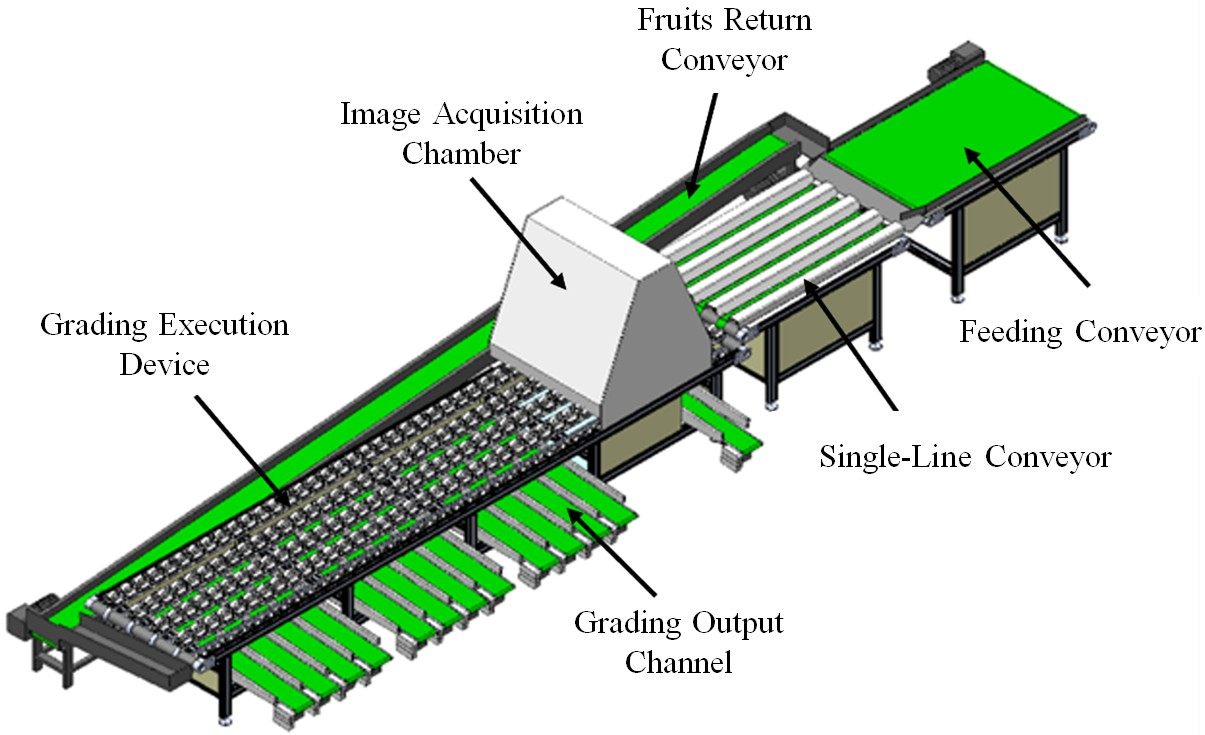
\includegraphics[width=0.7\linewidth]{figures/Bu2025}
	\caption{Mechanical model for the Orah sorting line \citep{bu2025grading}}
	\label{fig:Bu2025}
\end{figure}

\sectionsubsub{Transfer-learning based multi-class areca nut image classification under uncontrolled lighting on a conveyor system for automated sorting}
The study developed a conveyor-based system for the automated sorting of areca nuts based on ripeness, utilizing transfer learning for multi-class image classification under challenging, uncontrolled ambient lighting conditions. The system consisted of a feeder-scooper to singulate nuts, a conveyor belt with a green backdrop and black strips to prevent rolling, a five kg-cm torque stepper motor, and an imaging station with a RGB camera, triggered by an IR sensor. The core challenge addressed was classifying areca nuts into three market-relevant ripeness categories—Green, Green-Yellow, and Orange—based on a dataset of 1,615 images. The authors investigated the impact of different image pre-processing techniques, creating four dataset versions: the original, manually cropped, and two sets cropped automatically using contour detection and Hough circle transforms with different thresholds. Four pre-trained CNN architectures—Inception V3, ResNet50, InceptionResNetV2, and VGG16—were fine-tuned and evaluated under different hyperparameters, including two learning rates (0.001 and 0.0001) and two dataset splits of 60-20-20 and 80-10-10. The key findings revealed that Inception V3 consistently delivered the best performance, achieving a peak testing accuracy of 91.98\% and an F1 score of 0.92 using the original, uncropped dataset with an 80-10-10 split and a learning rate of 0.0001. InceptionResNetV2 achieved 90.74\% accuracy, VGG16 achieved 88.27\%, and ResNet50 performed poorly at 68.52\%. A critical discovery was that all cropping methods reduced model accuracy; for example, Inception-V3’s accuracy dropped to 84.47\% with manual cropping. VGG16 was particularly sensitive, with its F1 score falling from 0.833 on the original dataset to 0.516 on the manually cropped set \citep{kumar2024transfer}.

Table \ref{tab:relatedstudies_one} shows the comparison of the studies presented above.

\newpage

\begin{sidewaystable}
	\centering
	\caption{Comparison of Automated Quality Grading and Sorting Systems}
	\label{tab:relatedstudies_one}
	\begin{tabular}{
			>{\centering\arraybackslash}m{2cm} 
			>{\centering\arraybackslash}m{3cm}   
			>{\centering\arraybackslash}m{1.5cm} 
			>{\centering\arraybackslash}m{3cm}    
			>{\centering\arraybackslash}m{3cm}  
			>{\centering\arraybackslash}m{4cm}  
		}
		\toprule
		\textbf{Author(s)} & \textbf{Conveyor System} & \textbf{Camera} & \textbf{Rotation Type} & \textbf{Sensor(s)} & \textbf{Sorting Actuator} \\
		\midrule
		
		\citet{liu2024design} &
		Fixed tray type &
		\checkmark &
		&
		Photoelectric sensor &
		Electromagnet-controlled turnouts \\
		
		\citet{xu2024design} &
		Rotating roller \& belt conveyor &
		\checkmark &
		Free rotation &
		IR sensor &
		Pneumatic cylinders \\
		
		\citet{xu2025research} &
		\checkmark &
		\checkmark &
		&
		&
		\\
		
		\citet{zhang2021development} &
		Pitch-variable screw conveyor &
		\checkmark &
		Free rotation &
		Gear-tooth speed sensor &
		Rotary solenoid and paddle sorter \\
		
		\citet{lee2023multi} &
		\checkmark &
		Three cameras &
		Controlled, regular rotation &
		Object detection sensor &
		Stepping motor \\
		
		\citet{hu2021infield} &
		\checkmark &
		Three cameras &
		&
		Photoelectric sensor &
		Push plate \\
		
		\citet{bu2025grading} &
		Cup-based sorting line &
		\checkmark &
		Free rotation &
		Photoelectric sensor &
		\\
		
		\citet{kumar2024transfer} &
		\checkmark &
		\checkmark &
		&
		IR sensor &
		\\
		
		\bottomrule
	\end{tabular}
\end{sidewaystable}

\newpage

\subsection{Image Processing Techniques for Quality Assessment of Agricultural Produce}
Image processing techniques play a pivotal role in the development of automated fruit and vegetable quality detection systems, enabling the non-invasive assessment of external characteristics such as defects, color, size, and shape. These techniques involve the application of algorithms for image enhancement, noise reduction, edge detection, and morphological operations, ensuring that critical quality attributes are effectively isolated and quantified for analysis. Related studies in this field investigate innovative approaches that combine these image processing methods with machine learning and deep learning models to address challenges such as varying produce appearance, complex defect patterns, and the need for real-time, high-accuracy grading in industrial settings.

\newpage

\begin{sidewaystable}
	\centering
	\caption{Comparison of Image Processing Techniques for Quality Assessment of Agricultural Produce}
	\label{tab:relatedstudies_two}
	\begin{tabular}{
			>{\centering\arraybackslash}m{3cm} 
			>{\centering\arraybackslash}m{2.5cm}   
			>{\centering\arraybackslash}m{2cm} 
			>{\centering\arraybackslash}m{2cm}    
			>{\centering\arraybackslash}m{2cm}  
			>{\centering\arraybackslash}m{2cm}  
			>{\centering\arraybackslash}m{2.5cm}
		}
		\toprule
		\textbf{Author(s)} & \textbf{Otsu Thresholding} & \textbf{Edge Detection} & \textbf{Contour Analaysis} & \textbf{K-means Clustering} & \textbf{Watershed Algorithm} & \textbf{Morphological Operations} \\
		\midrule
		
		\citet{amna2023machine} &
		&
		&
		\checkmark	&
		&
		&
		\checkmark \\
		
		\citet{Doan2023} &
		\checkmark &
		\checkmark &
		\checkmark &
		&
		&
		\\
		
		\citet{Narendra2021} &
		&
		&
		&
		\checkmark &
		\checkmark &
		\\
		
		\citet{Kazi2023} &
		&
		&
		&
		\checkmark &
		&
		\\
		
		\citet{Luo2024} &
		\checkmark &
		\checkmark &
		&
		&
		&
		\checkmark \\
		
		\citet{Alqethami2022} &
		&
		&
		&
		\checkmark &
		&
		\\
		
		\citet{Javidan2023} &
		&
		\checkmark &
		&
		\checkmark &
		&
		\\
		
		\bottomrule
	\end{tabular}
\end{sidewaystable}

\newpage

\subsection{Feature Extraction and Classification  Techniques for Quality Assessment of Agricultural Produce}
The application of image processing for identifying defects in agricultural produce is a specialized and critical domain that builds directly upon the foundational research in plant disease detection. The field is broadly divided into traditional machine learning, which relies on hand-crafted features like color, shape and texture, and deep learning, where CNN-based models automatically learn features from data. The following studies illustrate this spectrum of approaches, highlighting key advancements in model architecture, the critical importance of data preparation, and the performance trade-offs between accuracy and speed that are essential for developing a robust, real-time inspection system.

\newpage

\begin{sidewaystable}
	\centering
	\caption{Comparison of Feature Extraction and Classification Techniques for Quality Assessment of Agricultural Produce}
	\label{tab:relatedstudies_three}
	\begin{tabular}{
			>{\centering\arraybackslash}m{2.5cm} 
			>{\centering\arraybackslash}m{5cm}   
			>{\centering\arraybackslash}m{4.5cm} 
			>{\centering\arraybackslash}m{7cm}   
		}
		\toprule
		\textbf{Author(s)} & \textbf{Feature Extraction} & \textbf{Deep Learning Feature Extraction Algorithms} & \textbf{ML Classifier(s)} \\
		\midrule
		
		\citet{haque2022deepnetwork} &
		&
		Inception v3, VGG16, VGG19, ResNet50, MobileNet, NasNetMobile &
		SVM \\
		
		\citet{Kursun2025} &
		&
		AlexNet &
		Random Forest \\
		
		\citet{Wang2024} &
		GLCM, Haralick Texture, DWT, Histogram of Oriented Gradient, Diffusion Map &
		&
		Decision Tree, Naive Bayes,  LDA, SVM , Bagging \\
		
		\citet{Mputu2024} &
		&
		MobileNetv2, Inceptionv3, ResNet50, and AlexNet &
		SVM, Random Forest, KNN \\
		
		\citet{Chandra2024} &
		HSV histogram, DWT, GLCM &
		&
		SVM \\
		
		\citet{Azadnia2023} &
		&
		Inception v3, ResNet50, Custom CNN &
		\\
		
		\citet{Iqbal2020} &
		Hu moments, Haralick Texture, Color Histogram &
		&
		Random Forest, Logistic Regression, KNN, Decision Tree, Naive Bayes, LDA, SVM \\
		
		\bottomrule
	\end{tabular}
\end{sidewaystable}

\newpage

\subsection{Synthesis}
A significant research gap has been identified in the automation of grading and sorting systems for elongated and curved agricultural produce, particularly eggplants. Most existing studies, such as those by \citep{xu2024design} and \citep{bu2025grading}, have been primarily focused on spherical or root-based crops like apples and sweet potatoes. Full-surface inspection was achieved by \citep{lee2023multi} using a three-camera rotational system; however, the method was limited to spherical fruits. Likewise, \citep{bu2025grading} and \citep{xu2024design} utilized single-camera, multi-view inspections with free rotation, which could not ensure complete surface coverage. In contrast, \citep{liu2024design} developed a machine vision system for the quality grading of cucumbers—an elongated type of produce—using a fixed-tray conveyor setup equipped with a single top-view camera and photoelectric sensors. While effective in determining the mass of the cucumber, the system lacked bottom-surface visibility, which is important in achieving full surface inspection for the accurate quality evaluation of the produce. Similarly, \citep{amna2023machine} implemented an image-based quality detection system for mangoes and tomatoes using a single top-view camera and servo-driven sorting mechanism. Although the approach achieved reliable classification for spherical produce, it did not enable complete visual inspection for elongated crops. 

To address these limitations, the present study proposes an automated eggplant grading and sorting system that utilizes machine learning algorithms for feature selection and classification. The system is implemented on a conveyor with a transparent imaging platform and a two-camera configuration, allowing simultaneous capture of the eggplant’s top and bottom surfaces to ensure comprehensive inspection and accurate quality grading. The summary of these highlights is summarized as shown in Table \ref{tab:synthesis}.

\newpage

\begin{sidewaystable}
	\centering
	\caption{Comparison of Related Studies on Automated Grading and Sorting Systems}
	\label{tab:synthesis}
	\begin{tabular}{
			>{\centering\arraybackslash}m{2.5cm} 
			>{\centering\arraybackslash}m{2.5cm}   
			>{\centering\arraybackslash}m{2.5cm} 
			>{\centering\arraybackslash}m{3cm}   
			>{\centering\arraybackslash}m{3cm}  
			>{\centering\arraybackslash}m{3cm}  
		}
		\toprule
		\textbf{Author(s)} & \textbf{Product} & \textbf{Multiview Inspection} & \textbf{Vision Method} & \textbf{Sorting Mechanism} & \textbf{Target Feature/Defect} \\
		\midrule
		
		\citet{xu2024design} &
		Sweetpotato &
		\checkmark &
		YOLOv8, BoT-SORT tracker &
		Pneumatic cylinder
		Surface defects, size \\
		
		\citet{bu2025grading} &
		Orah mandarin &
		\checkmark &
		Improved ShuffleNet\_v2 (ShuffleNet\_wogan) &
		&
		Appearance, diameter \\
		
		\citet{lee2023multi} &
		Apple &
		\checkmark &
		CNN with Knowledge Distillation &
		Stepping motor &
		Surface defects \\
		
		\citet{liu2024design} &
		Cucumber &
		&
		MassNet &
		Electromagnet-controlled turnouts &
		Mass \\
		
		\citet{amna2023machine} &
		Mango, Tomato &
		&
		Custom CNN &
		Servo motor &
		Surface defects \\
		
		\bottomrule
	\end{tabular}
\end{sidewaystable}

}